%% Proposal appendix
\vspace{15ex} % label
\chapter{Appendix}
\label{cha:appendix}

See Section \ref{sec:positioning} for background information.

This section shows benchmark results that were collected over a period of 30
days for Network, CPU, Memory, IO, and two data bases. The tests were executed
every 5 minutes to collect sustainable performance results, and we were careful
to not show the performance of our small iWe provider under a favorable light,
mainly for the IO tests.

We used a batch of simultaneous HTTPS transfers for bandwidth, and the sysbench
tool with two running threads for CPU, memory and IO. For the database tests we
used a customized version of the benchmark tools from the LevelDB project. The
source code is available on
github\footnote{https://github.com/petersenna/leveldb}.

The iWe provider we are evaluated had two home-grade servers, each with 16GB of
RAM, two SSD disks in RAID-1 and an i5-3320M CPU. The provider is connected to
the Internet over a 1Gbps fiber link. While this configuration is very small, it
allowed us to demonstrate that we can get similar levels of performance on the
lower end of the hardware spectrum.

\begin{figure}
\centering
\begin{subfigure}{.5\textwidth}
  \centering
  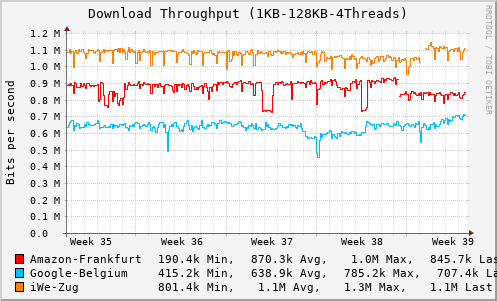
\includegraphics[width=0.98\textwidth]{30d-perf/download-month}
  \vspace{-0.05in}
  \caption{Download speed}
  \vspace{0.1in}
  \label{fig:sub1}
\end{subfigure}%
\begin{subfigure}{.5\textwidth}
  \centering
  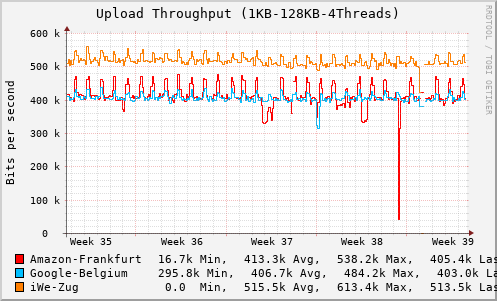
\includegraphics[width=0.98\textwidth]{30d-perf/upload-month}
  \vspace{-0.05in}
  \caption{Upload speed}
  \vspace{0.1in}
  \label{fig:sub2}
\end{subfigure}
\begin{subfigure}{.5\textwidth}
  \centering
  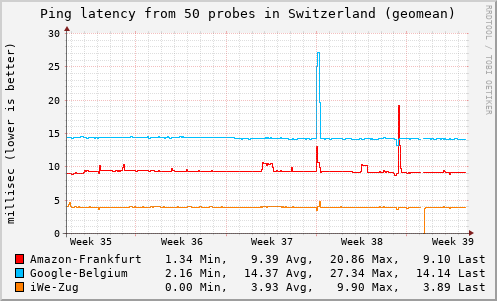
\includegraphics[width=0.98\textwidth]{30d-perf/ping-month}
  \vspace{-0.05in}
  \caption{Network latency}
  \vspace{0.1in}
  \label{fig:sub3}
\end{subfigure}%
\begin{subfigure}{.5\textwidth}
  \centering
  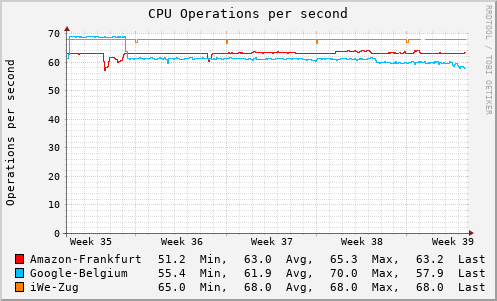
\includegraphics[width=0.98\textwidth]{30d-perf/cpu_ops-month}
  \vspace{-0.05in}
  \caption{Computing Power}
  \vspace{0.1in}
  \label{fig:sub4}
\end{subfigure}
\begin{subfigure}{.5\textwidth}
  \centering
  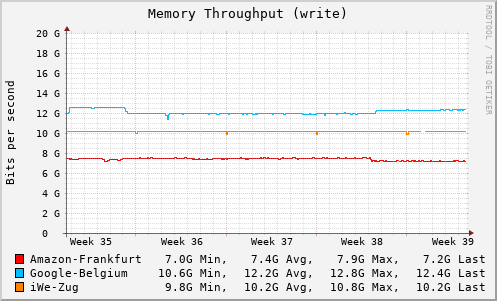
\includegraphics[width=0.98\textwidth]{30d-perf/mem_write-month}
  \vspace{-0.05in}
  \caption{Memory bandwidth}
  \vspace{0.1in}
  \label{fig:sub5}
\end{subfigure}%
\begin{subfigure}{.5\textwidth}
  \centering
  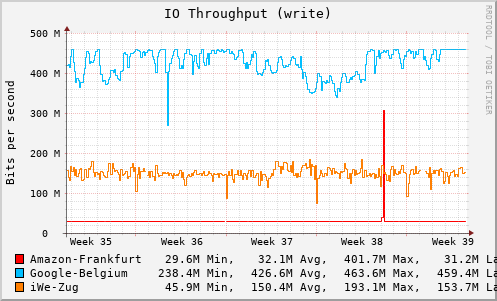
\includegraphics[width=0.98\textwidth]{30d-perf/io_write-month}
  \vspace{-0.05in}
  \caption{IO bandwidth}
  \vspace{0.1in}
  \label{fig:sub6}
\end{subfigure}
\begin{subfigure}{.5\textwidth}
  \centering
  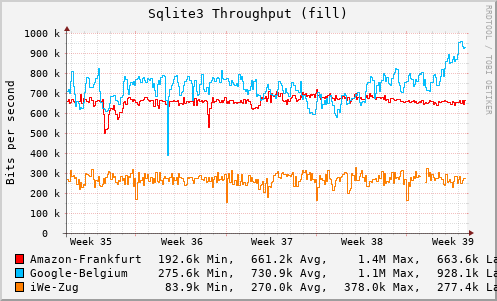
\includegraphics[width=0.98\textwidth]{30d-perf/sqlite3_fill-month}
  \vspace{-0.05in}
  \caption{SQLite3 write performance}
  \vspace{0.1in}
  \label{fig:sub7}
\end{subfigure}%
\begin{subfigure}{.5\textwidth}
  \centering
  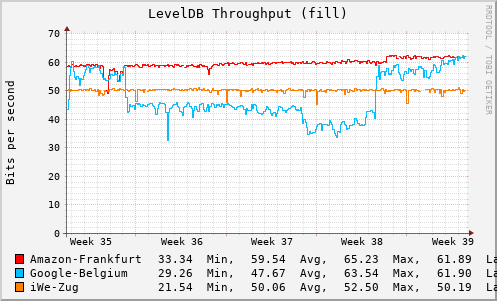
\includegraphics[width=0.98\textwidth]{30d-perf/leveldb_fill-month}
  \vspace{-0.05in}
  \caption{LevelDB write performance}
  \vspace{0.1in}
  \label{fig:sub8}
\end{subfigure}
  \caption{Performance Graphs}
  \label{graphs}
\end{figure}
\clearpage
